\problem{28}
{\sl Oxygen binding to myoglobin and hemoglobin}

Myoglobin and hemoglobin are proteins that bind oxygen in order to transport oxygen to
cells and tissues.
Myoglobin has a single subunit that binds a single oxygen; whereas, hemoglobin
is composed of four subunits that are each capable of binding an oxygen molecule.
In this problem, we address the binding of oxygen to myoglobin and hemoglobin
using a simple adsorption model (first developed by Linus Pauling).
The binding of oxygen to a subunit is associated with a favorable energy $-\epsilon$.
In the case of hemoglobin,
there is an additional favorable energy $-\delta$ of interaction when
oxygen are bound to adjacent sites.  Thus, the total energy for
2 bound oxygens is $-2 \epsilon - \delta$, and the total
energy for 3 bound oxygens is $-3 \epsilon - 3 \delta$.
The oxygen in the solution has a chemical potential 
$\mu = k_{B}T \log x +\mu_{0}$, where $x$ is the oxygen concentration.

\begin{figure}[h]\centering
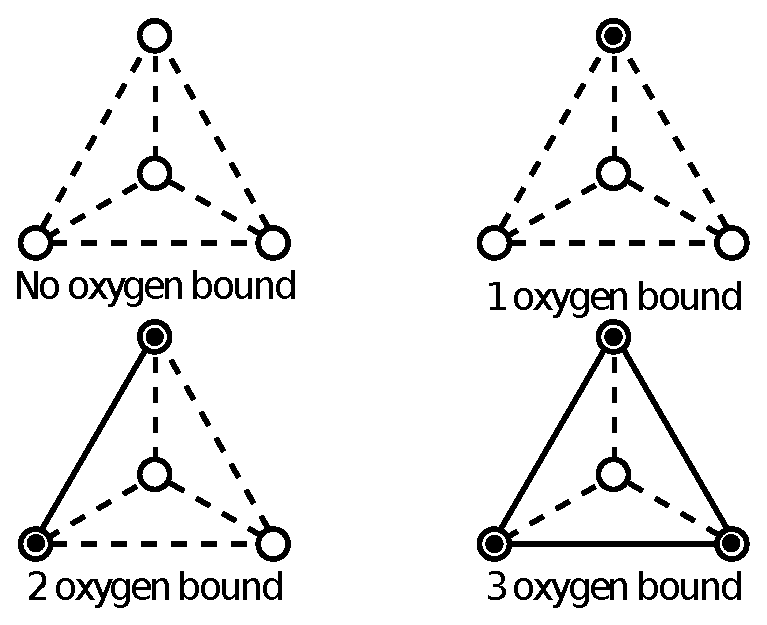
\includegraphics[width=0.4\textwidth,height=!]{hemoglobin}
\caption{\label{fig:hemoglobin}
Schematic of the Pauling model for oxygen binding to hemoglobin.}
\end{figure}

\smallskip\subp
Using a grand canonical ensemble, find the grand canonical partition function
$\Xi_\text{m}$ for the single-site model for myoglobin.

\smallskip\subp
Using an appropriate derivative, find an equation that governs
the average number of bound oxygen to myoglobin.

\smallskip\subp
Plot on a semilog scale the number of bound oxygens for the myoglobin model
versus the dimensionless concentration
$X=xe^{\beta \mu_{0}+\beta \epsilon}$.

\smallskip\subp
Using a grand canonical ensemble, find the grand canonical partition function
$\Xi_\text{h}$ for the 4-site model for hemoglobin.

\smallskip\subp
Using an appropriate derivative, find an equation that governs
the average number of bound oxygen to hemoglobin.

\smallskip\subp
Plot on a semilog scale the number of bound oxygens for the hemoglobin model
versus the dimensionless concentration
$X=xe^{\beta \mu_{0}+\beta \epsilon}$
for a dimensionless cooperativity factor $f=e^{\beta \delta}=1,2,5,10$.

\smallskip\subp
Describe in a couple of sentences how the
binding curves change with the cooperativity factor $f$.
Explain how the range of concentration where the oxygen
is released from the protein is affected by $f$.
What biological advantage is evident in homoglobin over
myoglobin?

\bigskip
\problem{12}
In class, we studied the partition function for diatomic molecules
in details, and calculated the partition function for the rotational degree of freedom
\begin{equation}
q_\text{rot} = 
\sum_{l=0}^\infty (2l+1) \exp\left[-\frac{\hbar^2}{2\mu R^2 \kB T}l(l+1)\right] 
\label{eq:qrot}
\end{equation}
by replacing the summation with integral over $l$.
We found that $q_\text{rot} \simeq T/\theta_\text{rot}$,
with $\theta_\text{rot} \equiv \frac{\hbar^2}{2\mu R^2 \kB}$.

\smallskip\subp
The above result can be systematically improved by using
the Euler-Mclaurin summation formula, which reads
$$ \sum_{n=a}^{b} f(n) = \int_a^b f(n)\, \dd n
+ \frac{f(a) + f(b)}{2}
- \frac{f^{(1)}(a) - f^{(1)}(b)}{12}
+ \frac{f^{(3)}(a) - f^{(3)}(b)}{720}
+ \cdots $$
where $f^{(1)}$ and $f^{(3)}$ are the first and third order derivatives.
Apply this formula to Eq.~(\ref{eq:qrot}) and show that
$$ q_\text{rot} =
\frac{T}{\theta_\text{rot}} + \frac{1}{3} + \frac{1}{15} \frac{\theta_\text{rot}}{T} +
\mathcal{O}\left(\frac{\theta_\text{rot}^2}{T^2}\right) $$

\smallskip\subp
Using the above result to calculate the error involved by
using $q_\text{rot} \simeq T/\theta_\text{rot}$ for
(1) $\rm N_2$\,(g) at 300\,K;
and (2) $\rm H_2$\,(g) at 300\,K.
The reduced mass $\mu$ for diatomic molecule is calculated by using
$\mu = m_1 m_2 / (m_1 + m_2)$, where $m_1$ and $m_2$ are the mass of two composing atoms.
The interatomic distance $R$ is $1.094$\,\AA\ for $\rm N_2$ and
is $0.742$\,\AA\ for $\rm H_2$.

\smallskip\subp
The previous calculations demonstrate that at normal condition
the rotational modes have all been excited.
So the temperature dependence to heat capacity comes mainly from the vibrational modes.
A set of experimental heat capacity values for CO\,(g)
over the temperature range $300\,{\rm K} < T < 1500\, {\rm K}$
is tabulated below.
$$\begin{array}{rc}
T/{\rm K} & C_V/(N \kB) \\
\hline
  300 & 2.455 \\
  400 & 2.538 \\
  500 & 2.621 \\
  600 & 2.689 \\
  700 & 2.764 \\
  800 & 2.833 \\
  900 & 2.928 \\
 1000 & 2.992 \\
 1100 & 3.019 \\
 1200 & 3.107 \\
 1300 & 3.154 \\
 1400 & 3.221 \\
 1500 & 3.243 \\
\end{array}$$
%$$ \frac{C_\text{V}}{N\kB} = 2.192 + (9.240\times10^{-4}{\rm K^{-1}})T 
%- (1.41\times10^{-7}{\rm K^{-2}})T^2 $$
%Plot $C_\text{V}/(N\kB)$ versus $T$ over this range,
Estimate the vibrational temperature $\theta_\text{vib}$ for CO\,(g) by fitting the above
data to the prediction of the result derived in class:
$$ \frac{C_\text{V}}{N\kB} = \frac{5}{2} +
\left(\frac{\theta_\text{vib}}{T}\right)^2 \frac{\ee^{-\theta_\text{vib}/T}}
{(1 - \ee^{-\theta_\text{vib}/T})^2} .$$
Report your fitted value for $\theta_\text{vib}$ and plot
experimental data and prediction on a single graph.
({\sl Note: The vibrational temperature for CO is $\theta_\text{vib} = 3107\,$K.})

\bigskip
\problem5
Shannon (1948) perceived that entropy quantifies the ignorance of possible observations
made to a system, and
showed that the Gibbs entropy expression we discussed in class can be used to
calculate this ``ignorance'':
$$ I = - \sum_n p_n \log_2\, p_n .$$
Here $n$ is a possible outcome of a single measurement,
and $p_n$ the corresponding probability.
$I$ is the average information, in unit of {\bf bit},
gathered after an observation or measurement has been made.
(He used the base-2 log for information whereas we used base-$\ee$ for entropy.)
For the two-state model we studied in class,
using the above notation, we may say that at $T = +\infty$,
the information collected after measuring the energetic state of a single particle is
$$I(\text{two state}; T=+\infty) = -\frac{1}{2}\log_2\left(\frac{1}{2}\right)
- \frac{1}{2}\log_2\left(\frac{1}{2}\right) = 1 \,\text{bit},$$
as the particle sits in any of the two states with probability $1/2$.
At zero temperature ($T=+0$), measuring the state of particles provides 0\,bit of information,
since we know with certainty before any measurement that the
particles are all seated in the low-energy state (the third law).
Shannon applied this analysis to the statistics of words in English language,
and here is what he did.
He noticed the occurrence frequency of English word closely follows the Zipf's law
(see Fig.~\ref{fig:zipf})
$$ p_n = \frac{0.1}{n} .$$
Then he assumed that English language only has $n_\text{max} = 12367$ words---this is obviously an irritating assumption, but it is the cutoff value for $n$ such that
$\sum_{n=1}^{n_\text{max}} \frac{0.1}{n} = 1.000$.
This assumption essentially neglects the entropy from higher rank words.
\begin{figure}[h]\centering
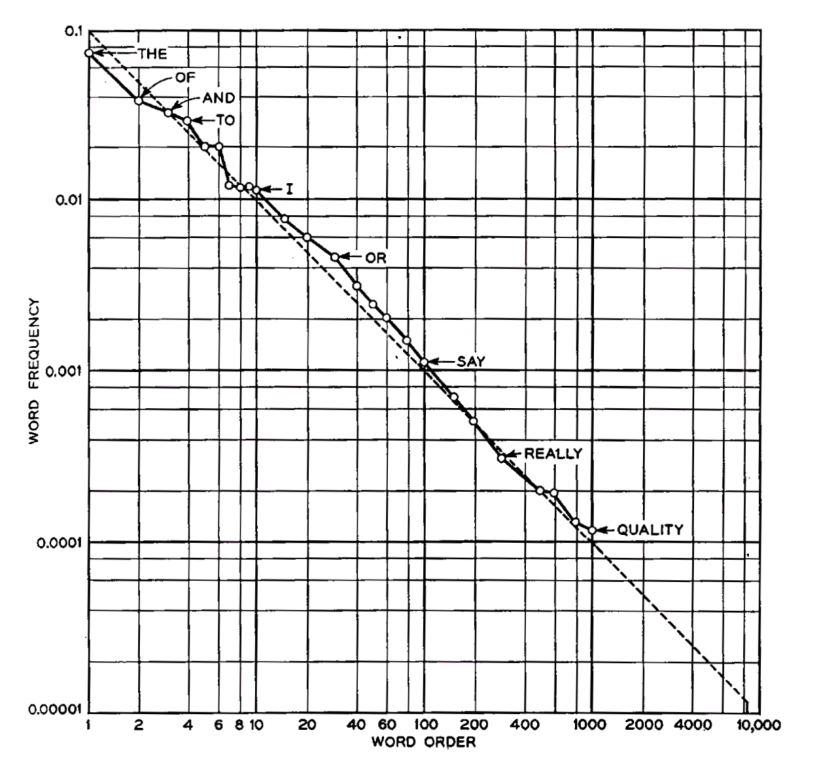
\includegraphics[width=0.618\textwidth,height=!]{zipf}
\caption{\label{fig:zipf}
Probability against frequency rank for English words.
The dashed line is the prediction of Zipf's law.
The most frequently used word is {\sl the};
the following ones are {\sl of}, {\sl and}, {\sl to}, etc.
}
\end{figure}

\noindent
Based on this assumption, compute the information bit $I$ per English word.
The average number of letter per English word is $5.1$ nowadays.
What is the information bit per English letter?
As a reference,
computer uses 8\,bits to store one letter.

